\documentclass[lettersize,journal]{IEEEtran}
\usepackage{amsmath,amsfonts}
\usepackage{algorithmic}
\usepackage{algorithm}
\usepackage{hyperref}
\usepackage{array}
\usepackage[caption=false,font=normalsize,labelfont=sf,textfont=sf]{subfig}
\usepackage{textcomp}
\usepackage{stfloats}
\usepackage{url}
\usepackage{verbatim}
\usepackage{minted}
\usepackage{graphicx}
\usepackage{cite}
\hyphenation{op-tical net-works semi-conduc-tor IEEE-Xplore}
% updated with editorial comments 8/9/2021

\begin{document}

\title{Laboratorio 2: Interferencia Intersımbolo (ISI)}

\author{
    Diego Martin~\IEEEmembership{}, diego.martin@mail.udp.cl \\
    Bruno Rosales~\IEEEmembership{}, bruno.rosales@mail.udp.cl \\
    Guillermo Carreño~\IEEEmembership{}, guillermo.carreño@mail.udp.cl \\
    Escuela de Informática y Telecomunicaciones\\
    Universidad Diego Portales

    26 de Abril de 2025
}

        % <-this % stops a space
%\thanks{This paper was produced by the IEEE Publication Technology Group. They are in Piscataway, NJ.}% <-this % stops a space
%\thanks{Manuscript received April 19, 2021; revised August 16, 2021.}


% The paper headers
%\markboth{CIT2111: Comunicaciones Digitales, Semestre I 2022}%
%{Shell \MakeLowercase{\textit{et al.}}: A Sample Article Using IEEEtran.cls for IEEE Journals}

%\IEEEpubid{0000--0000/00\$00.00~\copyright~2021 IEEE}
% Remember, if you use this you must call \IEEEpubidadjcol in the second
% column for its text to clear the IEEEpubid mark.

\maketitle


\section{Introducción}\label{sec:introduccion}

En este laboratorio se abordó el análisis de señales en sistemas de comunicación digital mediante el estudio del pulso coseno alzado y su representación temporal y frecuencial. Se realizaron distintas simulaciones que permitieron visualizar cómo varía la forma del pulso y su respuesta en frecuencia al modificar el parámetro de roll-off ($\alpha$). Además, se generaron diagramas de ojo para observar el efecto de la interferencia entre símbolos (ISI), tanto en condiciones ideales como en presencia de ruido gaussiano blanco aditivo (AWGN).

Las actividades se llevaron a cabo implementando scripts en MATLAB, utilizando funciones de generación de señales, filtros y visualización gráfica. Se definieron distintos valores de $\alpha$ (0, 0.25, 0.75 y 1) para evaluar su impacto en la forma del pulso y en el desempeño de la transmisión en un sistema digital simulado. Para la parte final, se simuló la transmisión de una secuencia de bits utilizando codificación NRZ-L y se observaron los resultados mediante la construcción de diagramas de ojo con y sin ruido.

El laboratorio fue realizado íntegramente en MATLAB debido a su versatilidad en el procesamiento de señales y su capacidad para generar gráficos de alta calidad, facilitando el análisis visual de los resultados. También se utilizaron funciones específicas para modelar el canal, introducir ruido y representar las señales en tiempo y frecuencia.

Este experimento se realizó con el objetivo de comprender el comportamiento del pulso coseno alzado, su relevancia en la reducción de la ISI y la importancia de parámetros como el $\alpha$ o roll-off y el ruido del canal. Asimismo, se buscó reforzar los conceptos teóricos vistos en clase, relacionándolos con aplicaciones prácticas y visuales que permiten un mejor entendimiento del funcionamiento de los sistemas de comunicación digital.


\section{Metodología}\label{sec:metodologia}
De manera que se pueda resolver el laboratorio, se llevan a cabo las actividades previas, en donde se definen las siguientes variables de una señal pulso de coseno alzado y una respuesta al pulso en frecuencia, utilizando los valores $\alpha$=0, $\alpha$=0.25, $\alpha$=0.75 y  $\alpha$=1 para el roll-off. Los valores para la gráfica del pulso deben ser \textit{t} $\geq$ 0, y para la frecuencia deben encontrarse en el rango de -2\textit{B} $\leq$ $f$ $\leq$ 2\textit{B}.
\begin{minted}{matlab}
Ts = 1; % Tiempo de símbolo
t = linspace(0, 8*Ts, 1000);
f = linspace(-2/Ts, 2/Ts, 1000);
alphas = [0, 0.25, 0.75, 1];
colores = lines(length(alphas)); 
leyendas = strings(1, length(alphas)); 
\end{minted}
Una vez definidos los parámetros iniciales, se procede a construir y graficar el pulso del coseno alzado para los valores definidos de $\alpha$ (0, 0.25, 0.75, 1), con t $\geq$ 0. 
Esto se hace con el siguiente código:

\begin{figure}[H]
        \centering
        \includegraphics[width=\columnwidth]{Imagenes/Screenshot_4.png}
        \label{fig:a1}
        \caption{Pulso Coseno Alzado con $\alpha$=0, 0.25, 0.75, 1}
\end{figure}

Esto genera un gráfico con cuatro curvas de coseno alzado, las cuales solo difieren en el valor del roll-off o $\alpha$ que toman.


Una vez construido y graficado el pulso del coseno alzado, se construye y se grafica la respuesta en frecuencia al pulso, donde -2\textit{B} $\leq$ $f$ $\leq$ 2\textit{B}. Esto se hace con el siguiente código:

\begin{figure}[H]
        \centering
        \includegraphics[width=\columnwidth]{Imagenes/Screenshot_5.png}
        \label{fig:a1}
        \caption{Pulso Coseno Alzado con $\alpha$=0, 0.25, 0.75, 1}
\end{figure}
Luego para la parte final del laboratorio, se debe generar un diagrama de ojo para el pulso coseno alzado con los siguientes parámetros:
\begin{itemize}
    \item Una codificación de línea NRZ-L.
    \item $10^4$ bits.
    \item Canal con ruido Gaussiano blanco (AWGN)
    \item Mismos valores de $\alpha$ que en la actividad previa.
\end{itemize}
Para esta parte se utilizaron 2 códigos distintos, uno para generar el diagrama de ojo sin ruido gaussiano, y otro para el gráfico con ruido gaussiano. Ambos cumplen con las otras condiciones propuestas.

Código Sin ruido gaussiano:

\section{Resultados y Análisis}\label{sec:resultados}
\subsection{Actividad Previa}
A continuación se describen los resultados obtenidos a partir de los códigos de la actividad previa. Los gráficos generados pueden encontrarse en el repositorio de GitHub correspondiente a este laboratorio (ver sección de Referencias), bajo los siguientes nombres de archivo:

\begin{itemize}
    \item \texttt{Impulsos-0.jpg}: Pulso Coseno Alzado con $\alpha$=0, 0.25, 0.75, 1.
    \item \texttt{Frecuencias.jpg}: Respuesta en frecuencia del pulso coseno alzado.
\end{itemize}

El primer gráfico representa la respuesta del coseno alzado para diferentes valores del parámetro roll-off. La respuesta al impulso muestra cómo la utilización de estos pulsos permite reducir la Interferencia Intersímbolo (ISI) en sistemas de comunicación digital.
%%%%%%%%%%%%%%%%%%%%%%%%%%%%%%%%%%%%%%
La respuesta al impulso es la onda resultante de la transmisión de un impulso unitario a través de un canal de transmisión el cual está modelado por el pulso coseno alzado, donde se muestra cómo se podría evitar la ISI utilizando estos pulsos de coseno alzado.

La ISI o interferencia intersimbolos es la superposición de las muestras de señales recibidas , cuando el canal en el que son transmitidas presenta limitaciones en el ancho de banda. Esta superposición hace que los símbolos generen interferencia, lo que dificulta la interpretación de las señales.
Para disminuir el efecto de la ISI se puede utilizar el pulso de coseno alzado. Lo que hace este puslo es suavizar las colas de los impulsos que se transmiten y reduce la energía fuera de la banda de la señal. Esto ayuda a garantizar que los símbolos de las señales no generen interferencias entre sí y que la señal sea más fácil de comprender.
%%%%%%%%%%%%%%%%%%%%%%%%%%%%%%%%%%%%%%

\subsection{Actividad Presencial}
El gráfico para el diagrama de ojo, sin considerar el ruido gaussiano, fue generado y puede visualizarse en el repositorio de GitHub correspondiente a este laboratorio (ver sección de Referencias). La imagen está guardada bajo el nombre de archivo \texttt{OjoNoG.png}.

Para el diagrama de ojo con ruido gaussiano considerado, se hacen 4 gráficos distintos correspondiendo cada uno a los distintos $\alpha$.

Los resultados correspondientes a los diagramas de ojo fueron almacenados y pueden ser visualizados en el repositorio de GitHub asociado a este laboratorio (ver sección de Referencias). Las imágenes están disponibles bajo los siguientes nombres de archivo:

\begin{itemize}
    \item Diagrama de ojo con $\alpha = 0$: \texttt{alpha0.png}
    \item Diagrama de ojo con $\alpha = 0.25$: \texttt{alpha0\_25.png}
    \item Diagrama de ojo con $\alpha = 0.75$: \texttt{alpha0\_75.png}
    \item Diagrama de ojo con $\alpha = 1$: \texttt{alpha1.png}
\end{itemize}

Estos gráficos permiten observar visualmente cómo varía la apertura del diagrama de ojo en función del valor de $\alpha$, lo cual refleja el nivel de interferencia entre símbolos (ISI) presente en la señal.

\subsection{Preguntas 1}
¿Que significa cada parametro del diagrama de ojo?
El significado de cada parametro para crear este diagrama
de ojo corresponde a:
\begin{itemize}
    \item Codificacion de linea NRZ-L: Corresponde al nivel de
voltaje de la senal
    \item Bits: se selecciono un total de 10000 bits, esto indica el total de bits que se transmiten.
    \item Canal con ruido gaussiano blanco (AWGN): Corresponde
al ruido que genera interferencia en la senal, afecta 
notoriamente al diagrama creado
    \item Roll-off: Representa la tasa de caida de amplitud en
respuesta al filtro utilizado.
\end{itemize}

\subsection{Preguntas 2}
¿Que pasa con el diagrama de ojo si disminuye la
frecuencia de muestreo?

Reduce la calidad de la señal, lo cual se relaciona directamente con el teorema de Nyquist-Shannon. Este establece que la frecuencia de muestreo debe ser al menos el doble de la frecuencia de la señal original. Por lo tanto, si se disminuye la frecuencia de muestreo, se pierden detalles importantes, lo que impacta negativamente en el diagrama de ojo.

\subsection{Preguntas 3}
¿Que pasa con el diagrama de ojo si se modifica el
valor de $\alpha$?

Lo que sucede es porque el $\alpha$ o roll-off indica la tasa de disminución
de amplitud del espectro, en caso de variar este parámetro
influiría directamente en la capacidad del filtro para disminuir la 
Interferencia.
\begin{itemize}
    \item $\alpha$ pequeño
    \begin{itemize}
        \item Pulso más estrecho en frecuencia.
        \item Mayor duración temporal → más ISI → ojo más cerrado horizontalmente.
    \end{itemize}
    \item $\alpha$ grande
    \begin{itemize}
        \item Pulso más ancho en frecuencia.
        \item Mejor localizado en el tiempo → ojo más abierto pero mayor ancho de banda necesario.
    \end{itemize}
\end{itemize}
\section{Conclusiones}\label{sec:conclusiones}
En este laboratorio se abordó el problema de la interferencia entre símbolos (ISI) en los sistemas de comunicación digital. Se demostró cómo la ISI se genera debido a la superposición de los símbolos transmitidos y cómo puede mitigarse mediante técnicas de filtrado adecuadas. Uno de estos filtros es el coseno alzado, utilizado para suavizar la cola del pulso y disminuir la energía fuera de la banda de la señal. Se representaron tanto la respuesta al impulso como la respuesta en frecuencia del filtro de coseno alzado para distintos valores del parámetro roll-off, además del diagrama de ojo.

Para reducir este efecto, se aplicó la técnica de Nyquist, la cual establece el ancho de banda óptimo necesario para evitar la distorsión de la señal y prevenir que los símbolos se sobrepongan entre sí. Disminuir la ISI y emplear filtros adecuados, como el pulso de coseno alzado, resulta fundamental para mejorar la calidad de las señales recibidas y, por consiguiente, optimizar la comunicación.
\section{Referencias}\label{sec:referencias}

\href{https://github.com/BrunoTrone1/lab_com_dig_2}{Repositorio en GitHub}
\section{Anexos}\label{sec:anexos}
\begin{figure}[H]
    \centering
    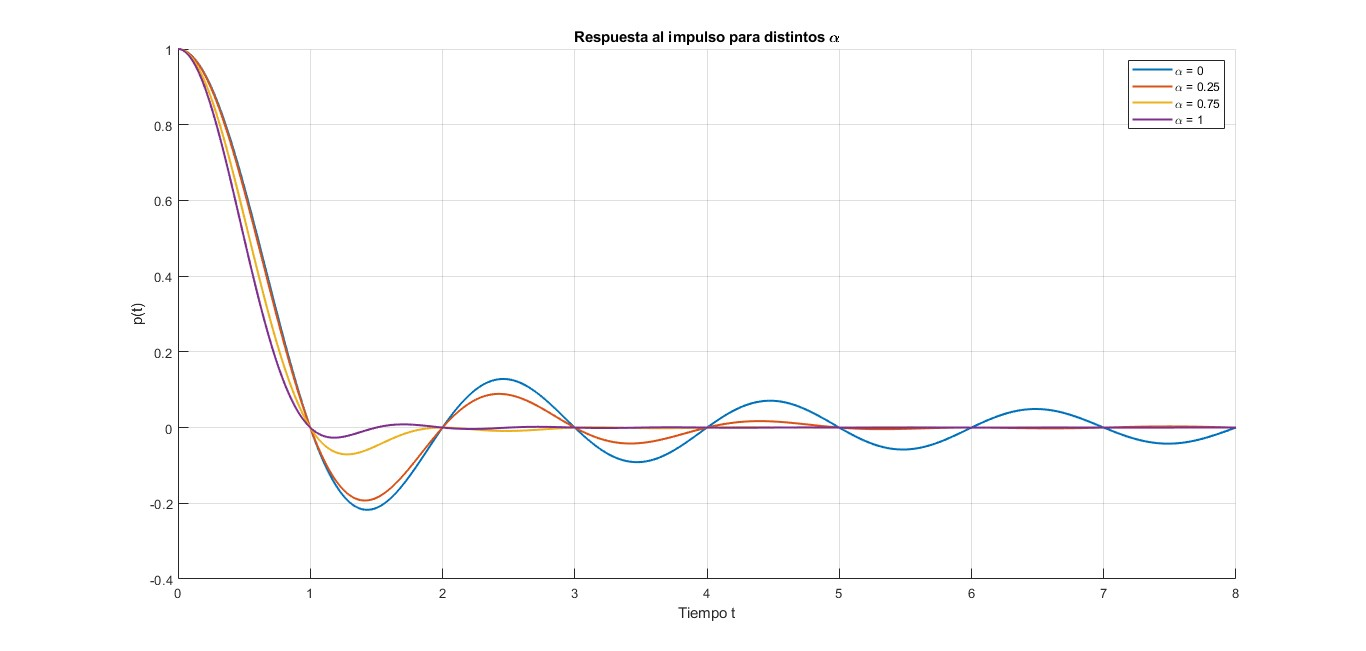
\includegraphics[width=\columnwidth]{Imagenes/Impulsos-0.jpg}
    \caption{Pulso Coseno Alzado con diferentes valores de $\alpha$}
    \label{fig:anexo1}
\end{figure}

\begin{figure}[H]
    \centering
    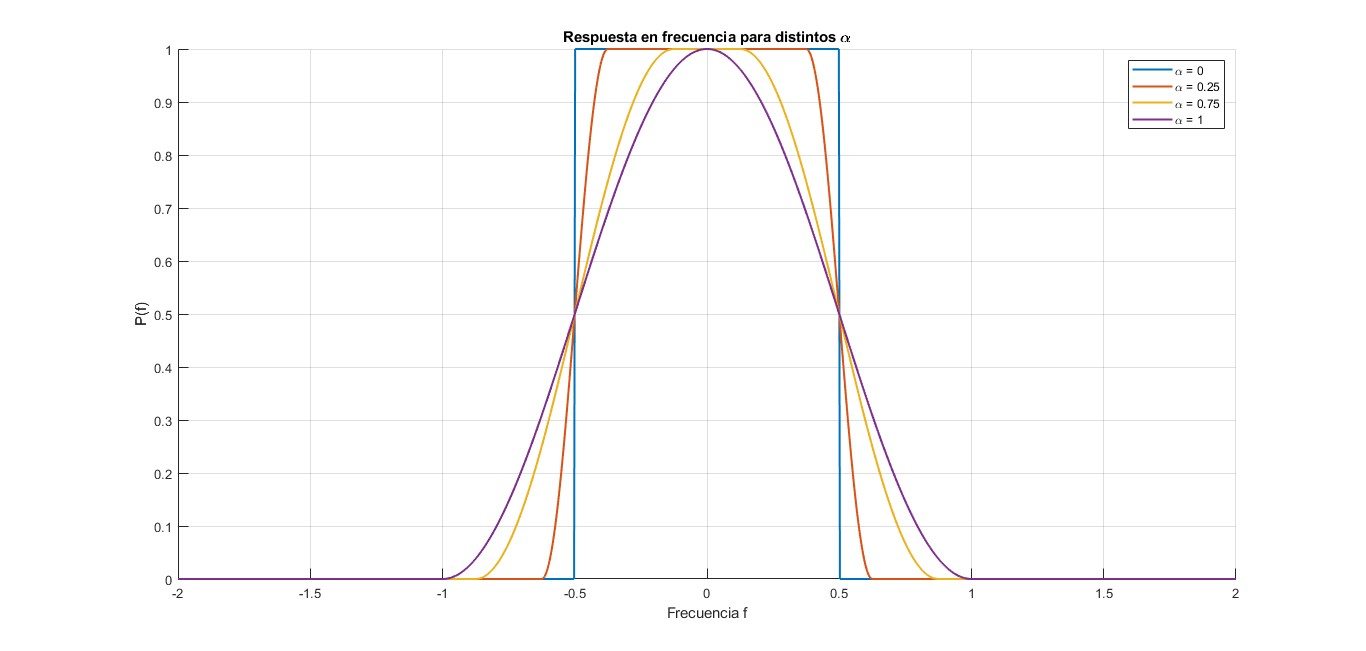
\includegraphics[width=\columnwidth]{Imagenes/Frecuencias.jpg}
    \caption{Respuesta en frecuencia del pulso coseno alzado}
    \label{fig:anexo2}
\end{figure}
\begin{thebibliography}{1}

\bibitem{IEEEhowto:kopka}
H.~Kopka and P.~W. Daly, \emph{A Guide to \LaTeX}, 3rd~ed.\hskip 1em plus
  0.5em minus 0.4em\relax Harlow, England: Addison-Wesley, 1999.

\end{thebibliography}


\end{document}
